\chapter{Background} % Main chapter title

\label{Chapter 2} % For referencing the chapter elsewhere, use \ref{Chapter 1} 

%----------------------------------------------------------------------------------------

% Define some commands to keep the formatting separated from the content 
\newcommand{\keyword}[1]{\textbf{#1}}
\newcommand{\tabhead}[1]{\textbf{#1}}
\newcommand{\code}[1]{\texttt{#1}}
\newcommand{\file}[1]{\texttt{\bfseries#1}}
\newcommand{\option}[1]{\texttt{\itshape#1}}

%----------------------------------------------------------------------------------------
\section{Neural Networks}

[Put in bit about perceptrons]

In 1959, Hubel and Wiesel discovered two kinds of cells in the primary visual cortex, a part of cerebral cortex that processes visual information, and their discovery entitled them the Nobel Prize 22 years later. They named those cells simple and complex cells based on difference in the conditions that caused the cells to fire. Loosely inspired by their work, Fukushima proposed an  neural network structure called the Neocognitron \cite{fukushima_neocognitron:_1982} [this is the wrong citation, the first paper out in 1980] in 1980. The Neocognitron is a multi-layer network with input and output layers as well as several hidden layers between them, alternating between hand-created convolutional recognition layers and pooling layers. Only adjacent layers are connected. The Neocognitron was able to recognize digits despite shifts in in the digits' positions and distortion in digits' shapes. 

Separately, in 1982, researchers proposed the "backpropagation" algorithm for the supervised training of general multilayer neural networks. [Add citations, look here for them: https://en.wikipedia.org/wiki/Backpropagation]   Specifically, backpropagation is an algorithm to change the weights between neurons to perform gradient descent on a specified loss function.  The loss function is calculated at the output layer then distributed back through each layer to provide pseudo-errors for hidden layers. As a result, parameters in each layer can be trained with gradient descent optimizer.

 One common loss function \(L(W)\) is calculated with desired output \(l\) and network output \(y\) using mean sum of squares, i.e. \(L(W) = \frac{1}{2n}\sum_{i = 1}^{n} (y_{i}-l_{i})^2\). Another commonly used loss function is called cross entropy, i.e. \(L(W) = -\sum_{i} l_{i}log(y_{i})\). Whatever the loss function, network parameters are updated in the direction which minimizes the loss function, i.e. \(W_{n+1} = W_{n} - \eta\nabla L(W_{n})\), where \(\nabla\) is the gradient operation and \(\eta\) is a scalar called learning rate. 

%----------------------------------------------------------------------------------------

\section{Convolutional Neural Networks}

Convolutional neural networks (CNNs) were first proposed by Yann LeCun et al. \cite{lecun_gradient-based_1998} in 1998. Compared to regular neural networks, convolutional neural networks take advantage of the spatial information from inputs and are easier to be trained due to the local connectivity property. Unlike the Neocognitron, the weights in CNNs are trained with supervised learning algorithms such as backpropagation.

All in all, convolutional neural networks are a type of deep models with multiple layers in which convolutional layers with trainable filters and local neighborhood pooling layers which decrease the dimension of output information are applied alternatively on raw input images, resulting in a hierarchy of increasingly summarized features \cite{ji_3d_2013}. 

[I am concerned that the above paragraph may be too close to the text you were reading at the time.]

A convolutional neural network usually contains several convolutional layers alternating with pooling layers and fully-connected layers. A simple example of a convolutional layer is given in Figure \ref{fig:cnn}. 

\begin{figure}[th]
\centering
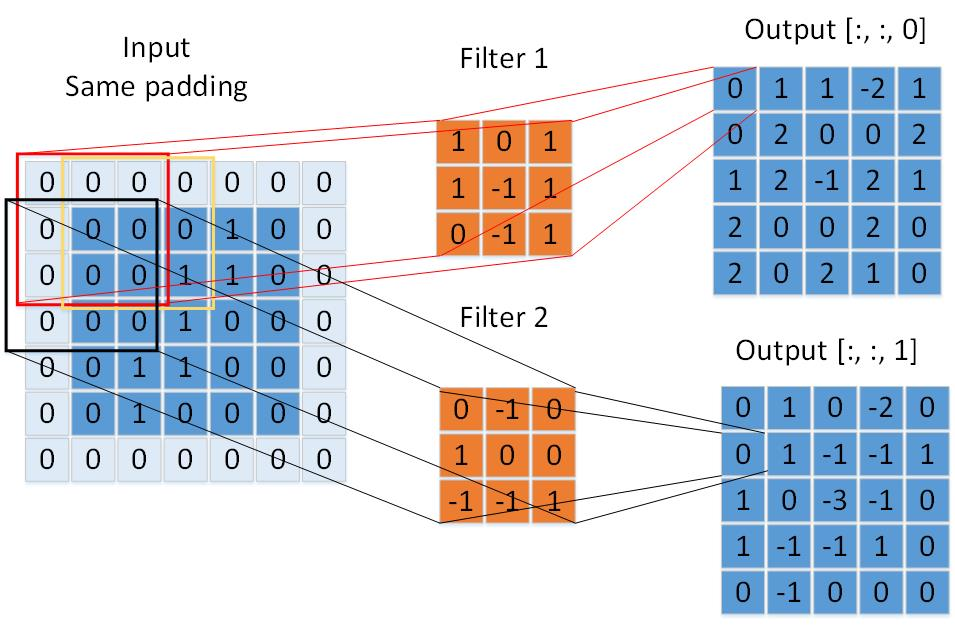
\includegraphics[width=80mm]{Figures/CNN}
\decoRule
\caption{A toy example of convolutional layer: same padding is used to maintain spatial dimension by adding zeros surrounding the original image. Element-wise multiplication then summation is done between the red square and filter 1 to obtain the value of the left-upper coordinate in the first layer of the output. The stride is 1 in this case, meaning the red square will next stride into the position of yellow square then same calculation is done between the yellow square and the filter 1. The value of coordinate located in the first row second column and first layer of output is obtained. The value of coordinate located in the second row first column in first layer of output is obtained using black square and filter 1. The second layer of the output is obtained with the second filter.}
\label{fig:cnn}
\end{figure}

Convolutional neural networks take matrices and tensors as inputs and do not reshape them into vectors, therefore preserving spatial information. The convolutional layers compute outputs using filters and a small region they are connected to in the inputs. Typically, neurons in CNNs are rectified linear units (ReLU), with the activation function  \(f(x) = max(x, 0)\). Here, for clarity, we describe the rectification step as a separate layer in the network.

Convolution layers in CNNs are usually followed by pooling layers. One common type is the \(2 \times 2\) max-pooling layer which takes the maximal value of each \(2 \times 2\) non-overlapping adjacent matrix. Pooling layers down-sample along the spatial dimensions, resulting in more summarized information. An example of ReLU layer and \(2 \times 2\) max-pooling layer is shown in figure \ref{fig:cnn2}. 

Finally, fully-connected layers are usually located at the end of CNNs, connecting them to the outputs. 

\begin{figure}[th]
\centering
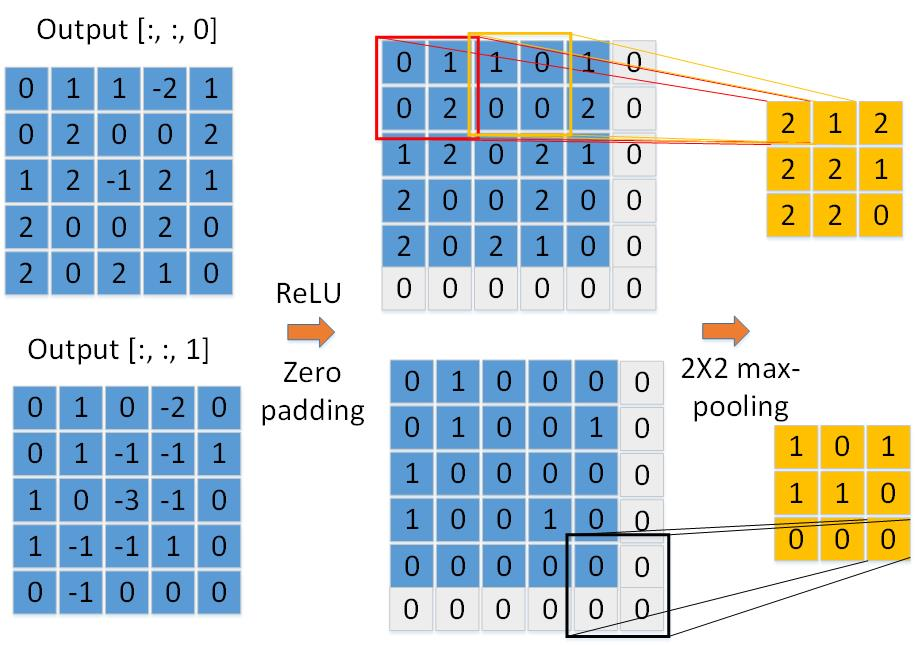
\includegraphics[width=80mm]{Figures/CNN2}
\decoRule
\caption{ReLU layer and \(2 \times 2\) max-pooling layer example following the toy example.}
\label{fig:cnn2}
\end{figure}



%----------------------------------------------------------------------------------------

\section{Autoencoders}

The concept of autoencoders was proposed by Rumelhart, Hinton and Williams in 1980s to address the problem of training without true labels \cite{rumelhart_learning_1985} [Fix this should be earlier, mention also autoassociators], which is also known as unsupervised learning. Unsupervised learning allows neural networks to detect statistical structure in their inputs even in the absence of labels. Because labeled data is often difficult to obtain, unsupervised learning plays an important role in the field of neural networks. Unsupervised learning is of particular interest in models of biological systems, since organisms must learn to accomplish visual tasks in the absence of any labeled inputs.

Autoencoders are multi-layer neural networks whose output layer has the same number of neurons as input layer. They are trainedto reproduce input information. Autoencoders take input \(x_{i} \in R^d, i = 1, 2...n\) and map the input to hidden layer \(h_{i} \in R^{d'}, i = 1, 2...n\) with the function \(h_{i} = \sigma(Wx_{i} + b)\), where \(W\) is the weight matrix and \(b\) is the bias vector in this encoder step. \(\sigma\) is the activation function in autoencoders. Autoencoders aim to reconstruct the input with function \(y_{i} = \sigma(W'h_{i} + b'), i = 1, 2...n\), where \(W'\) is the weight matrix and \(b'\) is the bias vector in this decoder step. Usually \(W' = W^T\) in order to reduce the number of parameters need to be trained \cite{masci_stacked_2011}. The autoencoder loss function is the mean sum of squares \(L = \frac{1}{2n}\sum_{i = 1}^{n} (x_{i}-y_{i})^2\).


Autoencoders are related to deep neural networks because training can be thought of as a special case of Contrastive Divergence [cite], the commonly used pretraining method for deep belief networks. As such, autoencoders are sometimes used in these pre-training steps. [citation here -- there is a paper that looks at this directly]. In this paper, we will show that the autoencoder pre-training process can by itself create a network that, when paired with a classification layer, performs accurately in digits recognition. 

%----------------------------------------------------------------------------------------

\section{Convolutional Autoencoders}

With the surprisingly accurate performance of convolutional neural networks in digit recognition [need citations here!], it was natural to introduce convolution into regular autoencoders. In 2011, Ciresan, Meier, Gambardella and Schmidhuber proposed a novel structure called convolutional autoencoders for unsurpervised feature extraction \cite{masci_stacked_2011}, which helped to achieve the best performance at the time in digit and object recognition. [is this true? Was it best in class at the time? I would be surprised!] The accuracy for a handwritten digits dataset call MNIST \cite{noauthor_mnist_nodate} is 99.29\%. [Is this the first time you mention MNIST? You should probably put it in earlier, when talking about CNNs or even before, and cite it there.] 

For input \(x_{i} \in {\rm I\!R}^d, i = 1, 2...n\), the latent k-th feature representation in an convolutional autoencoder is given by 
\begin{align}
h_{i}^k = \sigma(x_{i}*W^k+b^k)
\end{align}
where \(W^k\) is the filter for k-th feature and \(b^k\) is the corresponding bias vector. \(\sigma\) is the activation function and '*' stands for 2D convolution operation. Just as with regular autoencoders, the desired output of convolutional autoencoders is the output. The reconstruction is obtained by 
\begin{align}
y_i = \sigma(\sum_{k}{h_i}^k*\widetilde{W}^k + c)
\end{align}
where \(\widetilde{W}\) identifies the flip of \(W\), i.e. if \(W\) is of dimension [a, b, c, d] then \(\widetilde{W}\) is of dimension [b, a, d, c], and c is the bias vector \cite{masci_stacked_2011}. \(\sigma\) is the activation function and '*' stands for 2D convolution operation. The convolutional autoencoder loss function is still the mean sum of square
\begin{align}
E = \frac{1}{2n}\sum_{i = 1}^{n}(x_{i} - y_{i})^2
\end{align}
After training process, the encoder weight and bias will be used in original network to enable the corresponding layer to extract features for reproduction of inputs.

Pooling layers are often deployed after convolutional autoencoders in order to increase tolerance to input disturbance. [citations here]

%----------------------------------------------------------------------------------------

\section{Biologically Plausible Network Model}

CNNs may be a good model for biological visual processing. In the mammalian brain, visual information is believed to be processed hierarchically, passing from the retina through the thalamus to the visual cortical areas and finally arriving in the inferotemporal cortex \cite{burbank_understanding_2011}. The simple and complex cells first observed by Hubel and Wiesel can be found in each stage of the visual cortex, which raises the idea that the alternation of local filters with pooling structures seen in a CNN might be a good match for the this hierarchical visual processing. Moreover, the ReLU activation function typically used in CNNs is biologically plausible since biological neurons can only have positive levels of activity. The convolution operation itself, which allows the same filters to be used across multiple spatial locations, is likely not biologically plausible. However, the brain could learn similar filters in different locations by simply being exposed to similar visual stimuli at different locations over time. The convolution merely speeds up the process for training on the computer.


The difficulty in using CNNs as a biological model arrises from the training. Error backpropagation can train networks very successfully. However, error backpropagation among multiple layers is not currently believed to be biologically plausible. Backpropagation requires an error signal to be computed and passed backwards through the network at a time after a stimulus has been observed; this error signal is then multiplied with each neuron's prior activity to determine synaptic weight changes. But there is no good model for how such an error signal would be represented in neurons, how it could be segregated from ongoing feedforward activity, or how neurons could remember their previous activity in order to calculate the weight changes. As a result, a biologically plausible neural network model should avoid using error backpropagation among multiple layers. 

By contrast, biological models for layerwise autoencoder learning have been proposed. In particular, Burbank's model of mirrored spike-timing dependent plasticity \cite{burbank_mirrored_2015} showed how biologically realistic synaptic learning rules could lead a two-layered network of spiking neurons to implement the autoencoder learning rule. Here, we wish to test the effectiveness of multiple stacked autoencoders, trained layerwise, as a preprocessor for a final classification layer.
%----------------------------------------------------------------------------------------